%%%%%%%%%%%%%%%%%%%%%%%%%%%%%%%%%%%%%%%%
%   Original by                                   %
% Athanassios Protopapas, October 2005 %
% Mini-example for using apa.cls       %
%                                      %
% modified by William Revelle, August, 2007 
% modified by Irvin Hwang, January, 2010
%%%%%%%%%%%%%%%%%%%%%%%%%%%%%%%%%%%%%%%%

\documentclass[doc]{apa}%can be jou (for journal), man (manuscript) or doc (document)
%
%
%these next packages extend the apa class to allow for including statistical and graphic commands
\usepackage{url}   %this allows us to cite URLs in the text
\usepackage{graphicx}  %allows for graphic to float when doing jou or doc style
\usepackage{amssymb}  %use formatting tools  for math symbols
% type setting of functions, packages, and R follows a particular style
\let\proglang=\textsf
\newcommand{\R}{\proglang{R}}
\newcommand{\pkg}[1]{{\normalfont\fontseries{b}\selectfont #1}}
\newcommand{\Rfunction}[1]{{\texttt{#1}}} 
\newcommand{\fun}[1]{{\texttt{#1}}} 
\newcommand{\Robject}[1]{{\texttt{#1}}} 
%
%
%Here is where we start the important APA stuff
\title{Cognitive Prosem Proposal}
\author{Irvin Hwang}
\affiliation{Department of Psychology \\ Princeton University}

\ifapamodeman{%

\note{\begin{flushleft}

  Irvin Hwang\\

    Department of Psychology\\

  Princeton University\\

 Princeton, New Jersey\\

	08544\\

	e-mail: ihwang@princeton.edu\\

   

   \end{flushleft}}}

{%else, i.e., in jou and doc mode 

%\note{Draft of \today}
}


\shorttitle{Proposal}
\rightheader{Proposal}
\leftheader{Irvin Hwang}

\begin{document}
\maketitle   
\section{Specific Aims}
The broad theme of this work is to study how we acquire
domain-specific knowledge to model our environments.  More
specifically we look at how people distinguish features or patterns from the environment they are trying to model.

\subsection{Aim 1: Develop a theoretical framework for approaching problems that are not addressed by current theories of concept and statistical learning and mental models.}
The first aim of this project is to outline deficiencies in current theories and their abilities to explain how humans model their environment.  By looking at where these models fail, we aim to motivate and build upon an alternative theoretical framework that focuses on learning relationships in data and views computations as the basic unit of knowledge.  We plan to examine the problem of feature creation through the lens of this new theory.

\subsection{Aim 2: Combine insights gained from theory along with empirical evidence to develop a computational model of feature creation.}
The second aim of this work is to develop insights that will aid in
creating a computational model. The advantage of using a new framework is it
allows one to formulate classic questions as algorithmic problems and see if solutions are good models of behavior.  Finding good algorithms involves many design decisions that may be difficult to make analytically.  One way to approach these decisions is to create experiments that examine human behavior and try to extract nature's answer to these questions.  This work aims to apply both analytical and empirical approaches to the task of developing a computational model.


\section{Significance}
    It is clear the human endeavor of developing models is a cornerstone of scientific and more generally human progress.  On a less grandiose scale much of our ability to act intelligently in the world is possible because we develop knowledge of an environment/domain and apply it to achieve our goals.  Patterns and regularities in the world allow us to model our environment in an efficient manner and they are deeply ingrained in all fields of psychology.  At the perceptual level we deal with patterns such as shapes and textures to help identify objects.  Face recognition is a form of pattern processing that has important social influences.  The development of expertise in domains such as chess rely on the ability to recognize patterns of movements or strategies that improve the chances of winning.  The recognition of regularities in human behavior within different cultures is the basis for the development of stereotypes and prejudice.  The fundamental human ability of language involves recognizing patterns and structure.  Given the importance of modeling our world by recognizing patterns, it is important to understand the processes related to dealing with patterns.

\subsection{Concept learning}
The field of concepts and categories is arguably the most relevant area
of psychology related to the processes of abstract pattern recognition
and knowledge development.  The area deals with how we learn the to
categorize novel stimuli based upon known examples in a category \cite{bbc}.  One can interpret this process as learning the pattern of the data in a category well enough to be able to recognize that pattern in new data.  While concepts and categories is a relatively old field of cognitive psychology we point out a key limitation in the major theories and its importance to gaining a better understanding of our main themes.

The main idea of the prototype view is concepts/patterns are
represented as weighted feature lists and new items are categorized by
comparing similarity to each weighted feature list.  A
problem with this formulation of pattern recognition is demonstrated
by the concept of parity or generalized XOR i.e. when the stimuli are
bit strings and a particular string is labeled 1 if it contains an
even number of 1s otherwise it is labeled 0.  Since every bit is
equally important the weighted feature list representing the concept
should have equal weights for all the features.  The problem is the
prototypes for parity and non-parity categories are the same so
categorizing a new exemplar for either category cannot be based on
similarity.  One possible solution is to add the feature "even number
of bits" and put all weight onto this feature.  This raises crucial
questions prototype theory does not address such as where relevant features come from and how we define them. 

The main idea of exemplar theory is concepts are represented by
instances of stimuli/exemplars i.e. a set of feature lists as opposed
to a single weighted feature list.  A new exemplar is categorized by comparing similarity to the feature lists of each category.  Not only does the exemplar theory suffer the same limitations as the prototype theory due to its similarity based notion of concept, but it also does not have any ability to describe abstraction related phenomena.   Murphy \cite{bbc} gives an example of trying to understand flying squirrels as belonging to a flying/gliding category.  Since no exemplars of planes, birds, etc have the same folds a flying squirrel has "it is only by analogy or through a generalization of those exemplars that I can understand this new category...a more powerful inferential or abstraction mechanism would be needed."  One might argue that flying squirrels and the other exemplars of planes etc could have a feature indicating "wing-like" apparatus or "can fly" and this would make all the items in the category more similar, but the question of how this is determined is unclear from the theory.

The knowledge approach to concepts or "theory theory" is based on the
idea that prior knowledge has an effect on the learning of concepts.
Most of the focus in the knowledge approach research seems to be on
specific effects, but there have been connectionist models developed
by Heit and Bott \cite{bbc}.  Prior knowledge in these models is
essentially a hidden unit that is a combination of a subset of the
input features, but which features these should be is unclear.  In
general the architecture for such a network needs to be designed a
priori and if the input features are expected to be at the
sub-symbolic level such as pixels the question of architecture becomes
similar to the question of relevant features since once must know
which input features to combine and how to combine them to form
relevant prior knowledge.   

\subsection{Feature Learning}
    At this point it is clear the features involved in learning
    concepts are critical to the process and their origins are not
    well understood from current theory.  The work of Schyns and
    collaborators \cite{schyns98} seems to be the main line of
    research on feature creation and while they make a strong argument
    current theories of concept with fixed feature sets are
    incomplete, they have not produced models of feature creation and
    some problems with their theory arises from the lack of
    formalization.  The main statement they make about feature
    creation is it occurs when stimuli cannot be classified using the
    existing features.  The process of creating features is
    constrained by perceptual and functional biases and the history of
    categorization.  The authors argue against fixed features because
    any fixed set will be either too high level/structured or it will
    be too fine-grained.  In the case where the features are
    high-level or structured e.g. most feature sets in concept
    learning experiments, Biederman's geons, full shapes in vision
    etc. the set will undoubtedly not be flexible enough to capture
    reasonable patterns that are not combinations of the feature set.
    In the case of features being too fine-grained the authors argue
    certain abstract regularities such as symmetry, beauty, etc cannot
    be captured.  We argue this is not the case as the formation of abstract
    concepts from fine-grained features is possible when given access
    to a powerful enough language for expressing patterns.  We give a
    specific example later on.  Furthermore at some level any novel features must come from the raw sensory data at some point since this is ultimately the only source information about the external world.

A point the authors make worth noting is feature creation is
advantageous because it allows the elimination of complicated
categorization rules by the addition of new features citing XOR as an
example.  We believe this is not the complete story since the feature
they introduce is essentially determined through the computation that
would have been used on the original feature set in categorization.
The issue of feature creation is really the issue of finding
computations to represent relations or patterns between lower level features.
While the push for viewing features as a much more dynamic object and
something worth study in itself the authors' theory may be
inaccurate. 

\subsection{Statistical Learning}
One way to think of patterns and regularities in the environment is in
terms of statistics.  One approach in image statistics
\cite{Simoncelli01} starts with the distribution of natural or
artificial images then tries to discern properties of how the
statistics should be encoded based on the hypothesis of efficient
encoding.  We are interested in looking at patterns from any domain so
can we take this approach and generalize it to different situations?
One idea would be to estimate the distribution of the data using a
particular class of distributions and use something like MDL to
convert these distributions to a universal code for the data
\cite{MDLbook}.  The problem here is we must still estimate the
distribution and finding the proper class is similar to the problem of
finding a pattern in the data.  One might be able to use
non-parametric methods, but there are more fundamental problems such
as how one can take into account abstraction e.g. how data with
different surface features, but similar structure can share a common code.  One
major issue with optimizing compressibility is it is not clear
these codes necessarily retain any sort of semantics, which is
important since we often identify patterns based on their utility for
different tasks \cite{RossBFest}.  Ideally we would want a coding system where the
codes are meaningful e.g. summarizations of paragraphs into sentences.
Even when we do learn meaningful features e.g. horizontal lines or
facial parts etc using something like dimensionality reduction
techniques it is not clear whether one could encode complex relational
patterns as described earlier.  One might point to the work of
Torralba \cite{torr03}
using spectral signatures to classify different images of complex
objects, but it seems when one inspects the images you can determine
the categories from basic properties of the images rather than rich
relations on the features.  It is clear humans can automatically find
and characterize complex relations and statistical learning certainly
plays a part in this process, but the lack of an account for task
context and how the form of a pattern is determined and represented remain significant barriers.

At this point one might argue that features are the same as concepts
\cite{schyns98} and the question of feature origin can be answered
by current models of concept learning.  While concepts and features
may very well be the same, let us look at a concrete example as to why
current models cannot be a complete explanation of the origin
features.  Imagine the stimuli is as in Figure \ref{fig:stim}. 
\begin{figure}[htbp]
\begin{center}
%\includegraphics{fig275.pdf}
\includegraphics[scale=.2]{stim.pdf}
\caption{The top row consists of exemplars of the horizontal category
  and the bottom row is made up of non-horizontal exemplars. }
\label{fig:stim}
\end{center}
\end{figure}
The features are values of the pixels along with their coordinates and the concept we
need to learn is "horizontal" i.e. classifying lines that are
horizontal as different from those that are not.  
\begin{figure}[htbp]
\begin{center}
%\includegraphics{fig275.pdf}
\includegraphics[scale=.5]{both.pdf}
\caption{Imagine each box is many exemplars superimposed on each
  other. a) The left set is for the prototype model. The left box is a set from the horizontal exemplars and the
  right are non-horizontal exemplars. b) The right set is for the
  exemplar model.  The left box is a set from the horizontal exemplars and the
  right are non-horizontal exemplars plus a new stimuli in red. }
\label{fig:both}
\end{center}
\end{figure}
What happens we try to apply a prototype model?  Imagine the exemplars for the horizontal
concept consist of the set of horizontal rows and the exemplars for
non horizontal concept consist of the set of vertical columns \ref{fig:both}.
% \begin{figure}[htbp]
% \begin{center}
% %\includegraphics{fig275.pdf}
% \includegraphics[scale=.2]{proto.pdf}
% \caption{Imagine each box is many exemplars superimposed on each
%   other.  The left box is a set from the horizontal exemplars and the
%   right are non-horizontal exemplars. }
% \label{fig:proto}
% \end{center}
% \end{figure}
  Based on these exemplars both categories would have the same weighted
feature list representing their respective concept, which means
classifying a new exemplar would not be possible.  The problem is the
concept is independent of the concrete values of the features. 

This is further demonstrated when we try to apply an exemplar approach
to the problem.  Again we can choose a set of horizontal exemplars
such that they are all in one corner, A, and a non-horizontal in the
other corner, B, then present a new horizontal stimulus in corner B
overlapping the position of the non-horizontal stimulus \ref{fig:both}.
The model would categorize it as the non-horizontal concept since it has a better match with the non-horizontal exemplar.  
At this point one might say there is not enough information in the data for the
concept to be learned, but this is hardly true as it is probably
trivial for humans to learn facing this sort of problem.  The real
issue is the concept that needs to be learned is not a function of the
specific feature-values for exemplars i.e. cannot be computed based
directly on similarity, but rather it is the relationship between the
feature-values that is invariant.   The reason the models cannot learn
the concept is they are not able to compute or express this
relationship.  To see what we mean by this imagine we have a formal
system that can quantify over the features then one can express the
desired concept (informally) as there is a pixel with value 1, $p(x,y)=1$, such that
for $n>1$, $p(x+n,y)=1$.  If this expression is true for a stimulus then it
is categorized as horizontal and now we see that the cases in the
previous examples are no problem when we can express this relation.
While we used a problem from perception to illustrate our point the
real issue is domain independent.  The point is the concept is defined
by a relationship between features rather than as a computation on
specific feature values.  These "relational" concepts are not a
special pathological case, but in fact are more general than the
traditional concepts that have been studied in the past.  In some
sense almost all concepts/features must be relational since everything
must at some point be grounded in sensory data.    

The closest theories to addressing how relationships in data are learned
are the rule-based approaches such as rational rules or language of
thought research carried out by members of Joshua Tenenbaum's lab \cite{rrndg}\cite{KempGT07}.  This
line of work is similar to, but more advanced than Nosofsky's
rule-based concept learning research.  The main idea is the concept
learner has a language for expressing relationships in the data
e.g. first order predicate logic.  Expressions that represent
relationships are used to define categories.  A Bayesian approach is used to to integrate
the output for different expressions into a final category decision.
One way to interpret how learning is performed is to imagine a surface defined over the
space of all expressions in the language where the height of any point
(an expression in the language) is proportional to the performance of
the expression on the data (the likelihood).  Points on the surface are sampled such
that higher points (better expressions) are sampled more often i.e. carry more weight and the
weighted outputs of these expressions are
combined to form the final decision.  While the focus on finding
computable relations is the right direction there are a few major
problems that still need to be addressed.  The first is the theory
does not take into account for category use and context for which effects
have been demonstrated \cite{RossBFest}.  The second issue is the apparent
infeasability of Bayesian methods for finding good expressions.  The
space of expressions is huge and using the MCMC or similar Bayesian
approximation methods seems like applying generic search algorithms to
a hard problem.  Given enough time they will work, but due to their
generic nature they do not take advantage of the structure of the
problem.  One would not apply a generic Bayesian approach to a
discrete optimization problem like the packing problem or traveling
salesman and likewise one should attempt to find a more specific
algorithm for searching the space of expressions.  We provide a
framework that takes into account concept use and begins to probe the
issue of efficient methods for finding expressions.         

\section{Innovation}
We saw earlier one of the main limitations of current theories is the
inability of current models to express complex relations between
features.  Based on these observations we propose the beginnings of a
relation focused framework for understanding how humans recognize and use patterns
to model the world.  In the following section we present basic ideas
of the theory, give some examples of how one might think about formal
definitions, and examine questions that arise from this framework.

\subsection{Features, patterns, relations, and computation}
If the data we received from our senses was completely random, if the
world was random, we would be forced to keep all of it in order to
model our environment, but clearly this is not the case.  We can model
the world because it is not random.  We often refer to the
non-randomness or regularities as patterns and the presence or absence
or some other function of these patterns can be
understood as features of the data.  What does it mean for data to
have a pattern or not be random?
 
To get a more concrete sense of what we mean by pattern let us look at
a particular example (Figure \ref{fig:patterns}).  Suppose we have an image like the one below. 
\begin{figure}[htbp]
\begin{center}
%\includegraphics{fig275.pdf}
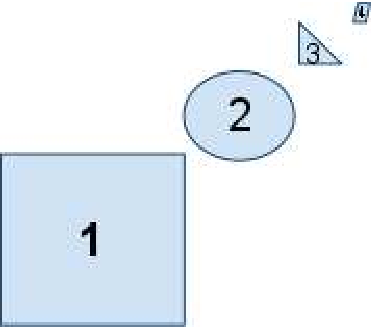
\includegraphics[scale=.5]{patterns.pdf}
\caption{This figure has a pattern of position and a pattern of size. }
\label{fig:patterns}
\end{center}
\end{figure}
This image is obviously not randomly generated and most people would
quickly recognize two patterns are present i.e. there are two features
1) the positions of the objects fall on a line and 2) they decrease in
size.  What does this mean more formally?  In the case of the first
pattern when we look at the centered position of the objects the
coordinates satisfy a linear relation represented by the computation
$y=mx+b$.  In the second case we see the relation $i<i+1$ holds where $i$ is
the area of the $i$th object.  In both cases we found that a computable
relation held for the data where data in the first pattern were object
positions and data in the second case were areas for the objects.  At
this point one might object to the use of symbols or "rules"
considering these patterns can be recognized without knowledge of the
formal equations.  The important thing to note is the relation that
defines the pattern exists independent of how it is represented and
computed.  Here we represented the relation by computations in a
formal system, but one can also imagine representing the same relation
as computations in a neural circuit etc.  From these examples we can
now define pattern recognition as finding computations summarizing a relation
that holds for the data. 

This formalization of patterns as relations leads to two natural
questions 1) what relations do we model in data and 2) how do we
choose the computations to represent a relation.  To begin developing
an answer to these questions we look at category use literature.
Brian Ross and collaborators have demonstrated "as one solves problems
over and over, one may learn different aspects of the problems that
could later become important in identifying and solving them,
especially by identifying properties that may not be evident through
superficial contact." \cite{bbc}.  So we find relations or features in data that
help us solve problems.  One way to formalize this is to think of life
in terms of a hierarchy of problems where the highest level is
survival e.g. The immediate problem I face is finding my car keys in
order to solve the problem of going to the grocery store, which is
part of the solution to making sure I get enough nutrients and this in
turn is a sub-problem for staying alive (individual survival can also
be thought of as a subproblem to species survival).  A domain can then
be defined as a sub-tree in this great tree of problems and modeling a
domain can be understood as finding the relations that lead to the
most solutions within the domain.  A solution to a problem can be
thought of as a sequence of actions that lead to a desired outcome.  One rough analogy to computer
science would be to think of solutions as algorithms and the
patterns/models mentioned earlier as abstract data structures in the
sense that the patterns guide what actions are possible on the data.
This leads to two possible criteria for search over the space of
relations and computations 1) the best relations (with respect to a
domain) are ones that lead to solutions for the most number of
problems 2)  The best set of computations is the minimal set required
to represent the best relations.

At this point it would be useful to clarify what we mean by
computation.  A computation is essentially any sort of transformation
on data.   There are many formal models of computation such as Turing
machines, the lambda calculus, etc. and there is a widely accepted
hypothesis that any computation (e.g. a computation made by a neural
network) can be expressed in terms of one of these formal models; this
is known as the Church-Turing thesis.  Perhaps the best way to think
about computations for our needs is as expressions in some programming
language.  So when we say the minimal set of computations for
representing a set of relations one can think of functions in a
language that are modular and can be reused in many different places.

We use an example of the concept of transitive set to demonstrate how
minimal computation can be a guiding constraint in finding patterns.
Imagine we have a set of numbers {1,2,3,...,n} and we have a
comparison operation that can compute whether one number is less than
another e.g. $1<2$, but $2 \not< 1$.  Using this operation we can
determine $1<2$, $1<3,...,1<n$, $2<3,...,2<n$,$3<n$ etc.  But we do not really
need all these computations.  By abstracting out the computation $a<b$
and $b<c \Rightarrow a<c$ directly from the data (possibly using a variant of a
string matching algorithm), we can combine it with the computations
$1<2$, $2<3$, $3<4$ to summarize the complete relation.  Once transitivity
is known one can use this information to develop efficient sorting
algorithms.  This is an example of how minimizing computation can lead to a description of a meaningful relationship.   

This may sound very different from work related to the mind, but to
help motivate these ideas we show how this view combined with the idea
that commonly performed computations get memoized (the results are
stored for quick access) leads to new interpretations of classic
effects in psychology (the following effects are described in \cite{bbc}).  Typicality is one of the main results in
classical concept learning.  The effect can be described as some items
in a category are more typical than others e.g. robins are more
typical than penguins.  One way to interpret this is the relations
defining the features for more common stimulus have had their
computations memoized so judging category membership (as in an
experiment by Rips,
Shoben, and Smith) for typical items is faster since the features
do not have to be recomputed.  The result of learning typical items of
a category faster can be interpreted in a similar fashion since the
features of typical items will be computed more often and thus
memoized.  Categories that require relational coding of features or
are not linearly separable have been better explained by an exemplar
model than a prototype model. These effects naturally lend themselves to the relation-based view
since it is based upon the learning of relations.  The relation based
framework also gives a more concrete definition of
knowledge where knowledge can be interpreted as previous the set of
computations made by a person and stored in memory.  The knowledge
effects of Pazzani (1991) as described by Murphy \cite{bbc}, which
describes how a disjunctive category of "the person must be an adult
OR the action must be stretching the balloon" was learned faster than
the conjunctive category "the color must be yellow AND the balloon
must be small" when cued with the task of identifying which balloon
would inflate.  The cue can be thought of as loading
computations/relations in the domain of inflating a balloon, which
would include the ones related to stretching the balloon and being an
adult so this would be learned faster.  In general it seems this relation-based
viewpoint is flexible enough at this level of detail to explain many
effects, but it remains to be seen whether it remains powerful once an
implementable model has been developed and the details have been
filled in.

The main barrier to developing a model of this view is the huge search
space of all computations that is involved.  One way to approach this
is by applying relatively generic algorithms such as Bayesian methods
combined with simulation techniques for approximating distributions.
We believe an approach that abstracts structure directly from the data
like in the example of transitivity is a more plausible approach.
While this example is far from enough to generate a complete theory
for the origin of relations/patterns/features we hope to use both
theoretical and empirical approaches to aid this goal.
\section{Approach}
\subsection{Overview}
Many questions arise from this theory and to address all of them would
be beyond the scope of this proposal.  One interesting question is
what patterns do people find over time in a domain when the goal is to
solve the most amount of problems in a set time.  We need to create many problems
within the same domain i.e. using the same objects; one way to do this
would be to look at solving algebraic equations.  A nice property of
the domain is there are clear relations that have utility in solving
certain problems e.g. $(a^2-b^2)=(a-b)(a+b)$ and we can generate
problems that need these relationships.  We can also keep track
of the number of operations a subject takes by having them record
their operations.  By having people solve sets of problems we can
observe the how they choose relations to use and how this changes over time.

\subsubsection{Participants}
Participants would be undergraduates from the university who can solve algebraic equations.  
\subsubsection{Design}
The experiment would consist of people solving a set of equations in
the least amount of time.  The
stimuli would consist of sets of nine equations with a particular
structure.  The structure is as follows.  The whole set of equations
would share a common relation that leads to non-optimal solutions for
each one.  The equations would also be divided into three sets of
three equations.  Each of these subsets would share a relation that
leads to a non-optimal solution and these solutions would be better
than the
ones that use the common relation to all equations.  Finally each
equation would have a unique relation that is needed to find the
optimal solution and this optimal solution would not use any of shared
relations.  Times for solving all the problems in each set would be
recorded as well as the operations used while solving each equation.
Subjects would solve sets until performance plateaus.

\subsubsection{Possible Outcomes}
We should be able to detect which relations subjects are using by
examining the operations for each equation.  We can then track the
order of the relations that are learned as the subjects solve more and
more sets.  We hypothesize people will learn the common relationships
first, which will initially allow them to solve more problems.  Once
they cannot increase their performance with this single relationship they
will learn the relationships at the next level and finally the unique
relationships for each equation.  

Potential problems with this approach would be generating the problems
with the required constraints.  One alternative would be to create an
artificial domain with all the properties we desire.  This would also
help us deal with prior familiarity of mathematical relations.

\subsection{Overview}
    Another question that arises from the theory is whether patterns processed in a top-down or bottom-up manner.  There are theories that are based upon locality assumptions and find small patterns first then attempt to find global relations between these patterns in a bottom-up process.  Evidence for a top-down approach comes from the field of expertise development where novices often start with an ability to identify coarse high level patterns, but with experience begin to decompose high-level patterns into collections of sub-features.  Understanding the direction of search would help develop the model because it could tell us whether computations for patterns should be built up from subexpressions or whether expressions for patterns should be refined and made more complicated when they do not accurately describe the data as a whole anymore.  How do we reconcile these two views?  One possibility is people try to apply patterns they already know at the level of coarseness relevant to problems they are dealing with and failing that they look for local patterns, which they can abstract and apply later.  An experiment to develop an understanding of these matters would be to look at the order of patterns recognized in complex stimuli such as long character strings.
\subsubsection{Participants}
Participants would be undergraduates from the university.  
\subsubsection{Design}
The experiment would consist of a learning phase then a test phase.  The stimuli would consist of strings with both coarse and local patterns e.g. 010232010232010232010232 here the course pattern has the form AAAA where A=010232 and the local pattern is of the form CDC where C=0 or 2 D=1 or 3.  One group would learn to classify stimuli based on coarse patterns while another group would learn to classify stimuli based on local patterns.  Once the groups have learned multiple patterns the test phase would begin.  In the test phase each group would have to learn a category based on a coarse pattern and a category based on a local pattern.  
\subsubsection{Possible Outcomes}
If the hypothesis holds each group should learn faster for their respective category e.g. the group trained on local patterns should learn the local test category faster.  If people learn patterns in a top-down fashion both groups should perform better on the coarse category and if people learn patterns in a bottom-up fashion then people should learn the category based on the local pattern faster.  One possibility is that certain patterns are more common than others so randomization should be used to control for prior knowledge.

\bibliography{psybib}
\end{document}
